\de{ĐỀ THI GIỮA HỌC KỲ I NĂM HỌC 2023-2024}{THPT Trường Chinh}
%%%==========================%%%
\begin{bt}%[0D1B1-3]%[Dự án đề kiểm tra toán khối 10-11 GHKI NH23-24-ThaiBao]%[Trường THPT Trường Trinh - TPHCM]
Lập mệnh đề phủ định mệnh đề sau và cho biết tính đúng sai của mệnh đề phủ định đó: Mệnh đề $P: " \forall x \in R: x ^2-4 x+4 < 0 "$
\loigiai{
	Mệnh đề phủ định của $P$ là:
$\overline{P}: \exists x \in R: x ^2-4 x+4 \geq 0$}.\\
Mệnh đề $\overline{P}$ là một mệnh đề đúng.\\ Thật vậy
$x ^2-4 x+4=(x-2)^2 \geq 0$.
\end{bt}
%%%==========================%%%
\begin{bt}%[0D1B2-1]%[Dự án đề kiểm tra toán khối 10-11 GHKI NH23-24-ThaiBao]%[Trường THPT Trường Trinh - TPHCM
	\begin{enumerate}
		\item  Cho tập hợp $E=\left\{{x} \in \mathbb{Z} |\left(2 x ^2-5 x+3\right)\left(x^2-9\right)=0\right\}$. Viết lại tập $E$ dưới dạng liệt kê và tìm tất cả các tập con của $E$
		\item  Cho hai tập hợp $A=[-4; 1)$ và $B=(-\infty; 0)$ Tìm $A\cap B, A\cup B, A\backslash B, C_{\mathbb{R}} A$
	\end{enumerate}
	\loigiai
	{\begin{enumerate}
	\item $E=\left\{-3;1;3\right\}$\\ Gọi $E_1,E_2,E_3,E_4,E_5,E_6,E_7,E_8$ là các tập con của tập hợp $E$, khi đó:\\
	$E_1=\left\{-3\right\}$, $E_2=\left\{1\right\}$, $E_3=\left\{3\right\}$, $E_4=\left\{-3;1\right\}$, $E_5=\left\{1;3\right\}$, $E_6=\left\{-3;3\right\}$, $E_7=\left\{-3;1;3\right\}$, $E_8=\varnothing$, 
	\item $A\cap B=[-4;0)$\\
	$A\cup B=(-\infty;1)$\\
	$A\backslash B=[0;1)$\\
	$C_{\mathbb{R}} A=(-\infty;-4)\cup[1;+\infty)$
	\end{enumerate}}
\end{bt}
%%%==========================%%%
\begin{bt}%[0D1K3-3]%[Dự án đề kiểm tra toán khối 10-11 GHKI NH23-24-ThaiBao]%[Trường THPT Trường Trinh - TPHCM
Lớp 10A có 45 học sinh trong đó có 14 bạn học sinh giỏi Toán, 17 bạn học sinh giỏi Lý, và 19 bạn không giỏi môn học nào trong hai môn Toán, Lý. Hỏi lớp 10A có bao nhiêu bạn học sinh vừa giỏi Toán vừa giỏi Lý?
\loigiai{
	Gọi $A$ là tập hợp học sinh giỏi Toán\\
	$B$ là tập hợp học sinh giỏi Lý\\
	$A\cap B$ là tập hợp học sinh giỏi cả hai môn.\\
	$n\left(A\cup B\right)=45-19=26$\\
	Tổng số học sinh giỏi môn Toán hoặc Lý là $14+17=31$\\
	Số học sinh giỏi cả hai môn là $n\left(A\cap B\right)=31-26=5$ học sinh.
}
\end{bt}
%%%==========================%%%
\begin{bt}%[0D2B1-2]%[Dự án đề kiểm tra toán khối 10-11 GHKI NH23-24-ThaiBao]%[Trường THPT Trường Trinh - TPHCM
Biểu diễn miền nghiệm của bất phương trình sau trên mặt phẳng tọa độ Oxy: $x+2 y-2 > 0$
\loigiai{
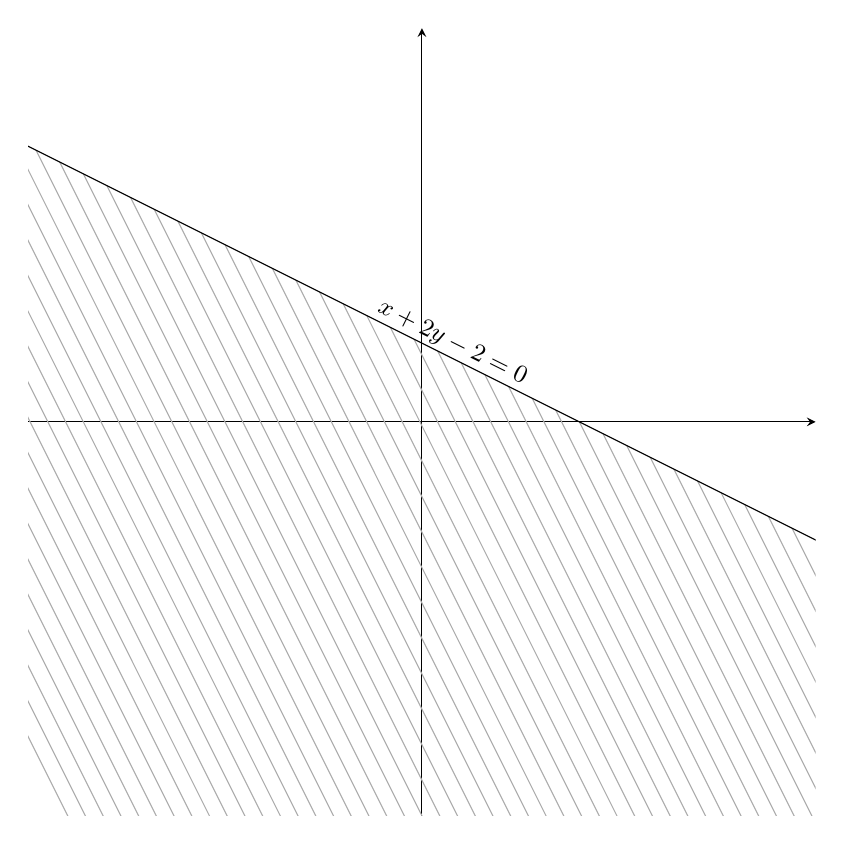
\begin{tikzpicture}[>=stealth,smooth,samples=100]
	\draw[->] (-5,0)--(5,0);
	\draw[->] (0,-5)--(0,5);
	\begin{scope}
		\clip (-5,-5) rectangle (5,5);
		%% Hàm thứ 1-----------------
		\pgfmathsetmacro{\goc}{abs(atan(0.5))-90}
		\foreach \i in {-10,-9.7,...,10}{
			\draw[gray!65,thin]({\i},{(-1*\i--2)/2})--+(\goc:15);}
		\draw plot[domain=-10:10]({\x},{(-1*\x--2)/2});
		\path (-1,1.5)--(1,0.5) node[sloped,pos=0.5,shift={({\goc+90}:11pt)},font=\small]{$x+2y-2 = 0$};
	\end{scope}
\end{tikzpicture}\\
Miền nghiệm là miền không tô và không kể bờ. }

\end{bt}
%%%==========================%%%
\begin{bt}%[0D2K2-2]%[Dự án đề kiểm tra toán khối 10-11 GHKI NH23-24-ThaiBao]%[Trường THPT Trường Trinh - TPHCM
Biểu diễn miền nghiệm của hệ bất phương trình: $\left\{\begin{array}{c}x+y+1 \leqslant 0 \\ x \geq 2\end{array}\right.$
\loigiai{
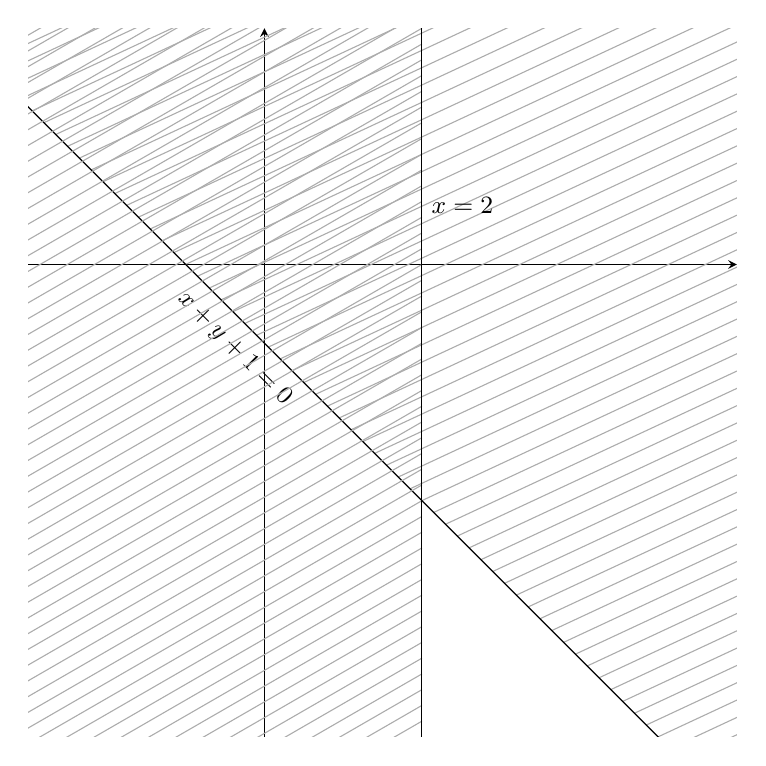
\begin{tikzpicture}[>=stealth,smooth,samples=100]
	\draw[->] (-3,0)--(6,0);
	\draw[->] (0,-6)--(0,3);
	\begin{scope}
		\clip (-3,-6) rectangle (6,3);
		%% Hàm thứ 1-----------------
		\pgfmathsetmacro{\goc}{abs(atan(1))-20}
		\foreach \i in {-10,-9.85,...,10}{
			\draw[gray!65,thin]({\i},{(-1*\i-1)/1})--+(\goc:15);}
		\draw plot[domain=-10:10]({\x},{(-1*\x-1)/1});
		\path (-1,0)--(1,-2) node[sloped,pos=0.5,shift={({\goc+210}:11pt)},font=\small]{$x + y+1 = 0$};
		%% Hàm thứ 2-----------------
		\pgfmathsetmacro{\goc}{210}
		\foreach \i in {-15,-14.8,...,20}{
			\draw[thin,gray!65]({-(-2)},{\i})--+(\goc:20);}
		\draw[variable=\t] plot[domain=-15:20]({-(-2)},{\t});
		\path (2,0.75) node[right,font=\small]{$ x= 2$};
	\end{scope}
	\end{tikzpicture}\\
Miền nghiệm là miền không tô và kể cả bờ. }
\end{bt}
%%%==========================%%%
\begin{bt}%[0H1K3-1]%[Dự án đề kiểm tra toán khối 10-11 GHKI NH23-24-ThaiBao]%[Trường THPT Trường Trinh - TPHCM
Cho tam giác $ABC$ có độ dài ba cạnh là $AB=2, BC=5, CA=6$
	\begin{enumerate}
		\item  Tính diện tích tam giác $ABC$ và độ dài đường cao kẻ từ $B$
		\item  Tính số đo góc B
	\end{enumerate}
	\loigiai{
	\begin{tikzpicture}[declare function={a=5;c=2;b=6;}]
	\path (0,0) coordinate (B)
	(5,0) coordinate (C);
	
	\path[name path=ca](B)circle(c);
	\path[name path=cb](C)circle(b);
	\path [name intersections={of= ca and cb, by={A,A'}}];
	\pgfresetboundingbox
		\path ($(A)!(B)!(C)$) coordinate (H);
	\draw (A)--(B)--(C)--cycle;\draw (B)--($(A)!(B)!(C)$);
	\foreach \t/\g in {A/90,B/180,C/90,H/90}{
		\draw[fill=white] (\t) circle (1pt) node[shift={(\g:7pt)},font=\normalsize]{$ \t $};
	}
		\path pic[draw,angle radius=5pt]{right angle= B--H--C};
	\path ($(A)!0.5!(B)$)coordinate(A')node[left,font=\normalsize]{$2$};
	\path ($(C)!0.5!(B)$)coordinate(B')node[below,font=\normalsize]{$5$};;
	\path ($(A)!0.5!(C)$)coordinate(C')node[above right,font=\normalsize]{$6$};;
	\end{tikzpicture}
\begin{enumerate}
	\item $p=\dfrac{2+6+5}{2}=\dfrac{13}{2}$\\
	$S_{ABC}=\sqrt{\dfrac{13}{2}.\left(\dfrac{13}{2}-2\right).\left(\dfrac{13}{2}-5\right).\left(\dfrac{13}{2}-6\right)}=\dfrac{3\sqrt{39}}{4}$.\\
	Gọi $H$ là hình chiếu vuông góc của $B$ lên $AC$. Khi này\\
	$S_{ABC}=\dfrac{1}{2}.BH.AC$\\
	$BH=\dfrac{2S_{ABC}}{AC}=\dfrac{2.\dfrac{3\sqrt{39}}{4}}{6}=\dfrac{\sqrt{39}}{4}$
	\item $\cos B=\dfrac{a^2+c^2-b^2}{2ac}=\dfrac{5^2+2^2-6^2}{2.5.2}=\dfrac{-7}{20}$
	$\Rightarrow \widehat{B}\approx110^\circ 29'$
\end{enumerate}
}
	
\end{bt}
%Câu 7...........................
\begin{bt}%[0H4K2-1]%[Dự án đề kiểm tra Toán 11 GHKI NH23-24- Dung Mai Dung]%[THPTTrường Chinh - Tp HCM]
	%Câu 7 (1 điểm) : 
	\immini{
		Để kéo dây điện từ cột điện vào nhà phải qua một cái ao, anh Nam không thể đo độ dài dây điện cần mua trực tiếp được nên đã làm như sau: Lấy một điểm $B$ như trong hình, người ta đo được độ dài từ $B$ đến $A$ (nhà) là $15 \mathrm{~m}$, từ $B$ đến $C$ (cột điện) là $18 \mathrm{~m}$ và $\widehat{A B C}=120^{\circ}$. Hãy tính độ dài dây điện $A C$ nối từ nhà ra đến cột điện.
	}{
		\begin{tikzpicture}[scale=0.3, every angle/.style={draw, angle eccentricity=1.2, angle radius=1cm}]
			% Định nghĩa các điểm
			\coordinate (B) at (0,0);
			\coordinate (A) at (15,0);
			% Tính toán vị trí của điểm C sử dụng quy tắc hàm cosin
			\coordinate (C) at ($(B) + (120:18)$);
			
			% Vẽ các cạnh tam giác
			\draw (A) -- node[below] {15m} (B) -- node[left] {18m} (C);
			
			% Vẽ các cạnh tam giác
			\draw[dashed] (C) -- (A);
			
			% Vẽ các góc
			\pic [draw, "$120^\circ$", angle eccentricity=1.5] {angle = A--B--C};
			
			% Đánh dấu các điểm
			\foreach \point in {A,C}
			\fill [black] (\point) circle (2pt) node[above right] {$\point$};
			\foreach \point in {B}
			\fill [black] (\point) circle (2pt) node[below] {$\point$};
			% Draw a black filled pentagon
			\filldraw[fill=black,opacity=.5] (4,4) -- (10,5) -- (15cm,15cm) -- (0cm,18cm) -- (-4cm,10cm) -- cycle;
			
		\end{tikzpicture}
	}
	\loigiai{
		Áp dụng định lý cosin trong tam giác $ABC$, ta có
		\begin{align*}
			AC^2 &= AB^2 + BC^2 - 2 \cdot AB \cdot BC \cdot \cos\widehat {ABC} \\
			AC^2 &= 15^2 + 18^2 - 2 \cdot 15 \cdot 18 \cdot \cos120^\circ\\
			AC^2 &= 15^2 + 18^2 - 2 \cdot 15 \cdot 18 \cdot \left(-\dfrac{1}{2}\right) \\
			AC^2 &= 225 + 324 + 270 = 819\\
			AC &= \sqrt{819} \approx 28{,}62\,\text{m}.
		\end{align*}
		Vậy độ dài của dây điện $AC$ là khoảng $28{,}62\,\text{m}$.
		
	}
\end{bt}
%Câu 8...........................
\begin{bt}%[0D2K2-3]%[Dự án đề kiểm tra Toán 11 GHKI NH23-24- Dung Mai Dung]%[THPTTrường Chinh - Tp HCM]
	Để có kinh phí làm từ thiện, CLB ầm thực trường THPT Trường Chinh có làm hai loại bánh flan và bánh rau câu để bán. Mỗi đợt sản phẩm bánh flan bán lãi 500 ngàn đồng, mỗi đợt bánh râu câu bán lãi 400 ngàn đồng. Để sản xuất được một đợt bánh flan nhóm I phải làm việc trong 3 giờ và nhóm II phải làm việc trong 1 giờ. Để sản xuất được một đợt bánh rau câu thì nhóm I phải làm việc trong 2 giờ và nhóm II cũng phải việc trong 2 giờ. Một nhóm không thể làm được đồng thời hai sản phẩm. Biết rằng trong một tuần nhóm $\mathrm{I}$ không thể làm việc quá 12 giờ và nhóm II không thể làm việc quá 8 giờ. Số tiền lãi lớn nhất trong một tuần của CLB ầm thực?
	\loigiai{
		Gọi $x$, $y$ lần lượt là số đợt sản xuất bánh flan và bánh rau câu. \\
		Ta có hệ điều kiện:
		\[
		\begin{cases}
			x \ge 0 \\
			y \ge 0 \\
			3x + 2y \le 12 \\
			x + 2y \le 8.
		\end{cases}
		\]
		\begin{center}
			\begin{tikzpicture}[>=stealth', x=1cm, y=1cm, scale=1]
				\def\xmin{-2} \def\xmax{5}
				\def\ymin{-2} \def\ymax{6}
				\clip(\xmin,\ymin) rectangle (\xmax,\ymax);
				\tkzDefPoints{\xmax/\ymax/A1,\xmin/\ymax/B1,\xmin/\ymin/C1,\xmax/\ymin/D1}
				\draw[->](\xmin,0)--(\xmax,0); \draw(\xmax-0.1,0) node[below]{$x$};
				\draw[->](0,\ymin)--(0,\ymax); \draw(0,\ymax-0.2) node[right]{$y$};
				\draw[smooth,samples=300] plot(\x,{-1.5*(\x)+6});
				\draw[smooth,samples=300] plot(\x,{-0.5*(\x)+4});
				%\draw[smooth,samples=300] plot(\x,{-2.02*(\x)+4.79});
				\foreach \ten/\x/\y in {A/0/4,B/2/3,C/4/0,O/0/0}{
					\coordinate (\ten) at (\x,\y);
				}
				\foreach \p/\r in {A/-70,B/-110,C/150,O/-120}
				\fill (\p) circle (1pt) node[shift={(\r:3mm)},scale=0.6]{$\p$};
				\fill[pattern=north east lines] (B1)--(0,6)--(0,\ymin)--(C1);
				\fill[pattern=north east lines] (0,6)--(A1)--(D1)--(C)--(B)--(A);
				\fill[pattern=north east lines] (0,0)--(\xmax,0)--(D1)--(0,\ymin);
				\foreach \p/\r in {1/1,2/2,3/3,4/4}
				\fill (0,\p) circle (0.5pt) node[shift={(180:5mm)}]{\small $\r$};
				\foreach \p/\r in {1/1,2/2,3/3,4/4}
				\fill (\p,0) circle (0.5pt) node[shift={(-90:5mm)}]{\small $\r$};
			\end{tikzpicture}
		\end{center}
		Miền nghiệm của hệ là tứ giác $OABCD$ với $A(0, 4)$, $B(2, 3)$, $C(4, 0)$.\\
		Lợi nhuận thu được là $F(x, y) = 500x + 400y$ (ngàn đồng).\\
		Giá trị của $F$ tại các đỉnh:
		\begin{itemize}
			\item \( F(0, 4) = 500 \cdot 0 + 400 \cdot 4 = 1600 \) ngàn đồng.
			\item \( F(2, 3) = 500 \cdot 2 + 400 \cdot 3 = 2600 \) ngàn đồng.
			\item \( F(4, 0) = 500 \cdot 4 + 400 \cdot 0 = 2000 \) ngàn đồng.
			\item \( F(0, 0) = 500 \cdot 0 + 400 \cdot 0 = 0 \) ngàn đồng.
		\end{itemize}
		Vậy để lợi nhuận tối đa, CLB ẩm thực cần sản xuất theo kế hoạch \( x = 2 \) đợt bánh flan và \( y = 3 \) đợt bánh rau câu, và lợi nhuận lớn nhất có thể đạt được là 2600 ngàn đồng.
	}
\end{bt}